% -----------------------------------------------------------------------------
% ------------------------------- PREAMBLE ------------------------------------
% -----------------------------------------------------------------------------[
	\documentclass[english]{scrartcl}

	\title{Spatial Complexity and Scaling in Cities}
	\subtitle{v0.0}
	\author{Phil Chodrow}
	\date{May 29th, 2016}

	\usepackage[T1]{fontenc}
	\usepackage[utf8]{inputenc}
	\usepackage{babel}
	\usepackage{blindtext}
	\usepackage{amsmath}
	\usepackage{amsthm}
	\usepackage{amsfonts}
	\usepackage{amssymb}
	\usepackage{enumitem}
	\usepackage{graphicx}
	\usepackage{pgfplotstable,filecontents}
	\usepackage{booktabs}
	\usepackage{caption}
	\usepackage{subcaption}
	\usepackage{csvsimple}

	\pgfplotsset{compat=1.9}% supress warning

	\setkomafont{disposition}{\normalfont\bfseries}

	\newtheorem{thm}{Theorem}
	\newtheorem{lm}{Lemma}
	\newtheorem{cor}{Corrolary}
	\newtheorem{clm}{Claim}
	\newtheorem*{thm*}{Theorem}
	\newtheorem*{lm*}{Lemma}
	\newtheorem*{cor*}{Corrolary}
	\newtheorem*{clm*}{Claim}
	\newtheorem*{fct*}{Fact}

	\newcommand\abs[1]{\left|#1\right|}
	\newcommand\E[0]{\mathbb{E}}
	\newcommand\R[0]{\mathbb{R}}
	\newcommand\decision[2]{\underset{#2}{\overset{#1}{\gtreqless}}}
	\newcommand{\argmax}{\operatornamewithlimits{argmax}}
	\newcommand{\argmin}{\operatornamewithlimits{argmin}}
	\newcommand\prob[0]{\mathbb{P}}
	\newcommand{\norm}[1]{\left\lVert#1\right\rVert}
% -----------------------------------------------------------------------------
% --------------------------------- BODY --------------------------------------
% -----------------------------------------------------------------------------
\begin{document}

\maketitle

\abstract{We formulate the \emph{mean local information}, a novel measure of spatial compositional complexity in terms of the localized mutual information between spatial and compositional variables. This measure is closely related to the Fisher information of the underlying joint distribution, and is therefore an intrinsic property of the phenomena studied. Using this measure, we study spatial variations in racial trends in major American cities. The results neatly distinguish cities with large, monoracial neighborhoods from those with more intricate, interleaved neighborhood structure. Furthermore, the mean local information scales logarithmically with population density, inviting future research into possible universal dynamical processes of neighborhood formation that might explain this relationship.}

\section{Introduction}

	Information theory provides one natural approach toward thinking about complex systems. It achieves this by mapping the physical concept of structure to the epistemic concept of predictability. A complex system has enough structure to be at least partially predictable, but enough disorder to make prediction challenging. In this paper, we apply information-theoretic tools to the measurement of \emph{spatial compositional complexity}, with a focus on the spatial variation of racial trends in American cities. 

	Information-theoretic concepts have already found application in urban planning problems related to zoning and predicting population distributions \cite{Royal2014,Batty1974,Batty1976,Battya}. Substantial recent work has addressed the measurement of difference and disparity in cities through an information-theoretic lens \cite{Theil1971,Bettencourt2015,Roberto2015a,Roberto2015}. Attractive features of information-theoretic measures for this purpose include their deep relationship to statistical inference \cite{Cover1991,Csiszzr2004}, their generalizability to multiple demographic phenomena, and the fact that Theil's (\cite{Theil1971}) original index satisfaction of many (though not all) of the invariance properties desirable for the measurement of segregation \cite{Reardon2002}. \nocite{Sampson2002,Dietz2002,Wong2004,Keeling1999,Anas1997,Ioannides2004a,Wong1999,Press2009a,Holloway2012,Lee2008,Louf2015}.

	While closely-related to segregation, the concept of complexity has received less attention among quantitative sociologists. This is natural, since complexity is both less operational than segregation and challenging to define. On the other hand, as we demonstrate below, a spatial information-theoretic measure can be defined which measures the granularity of neighborhood structure, distinguishing cities with large, monolithic tracts of constant racial composition from those with many adjacent, smaller, neighborhoods of varying racial profiles. In doing so, it therefore captures one natural aspect of complexity in spatial compositional phenomena, and may also be of interest as a segregation measure as well. 

\section{Information Theory and Spatial Structure}

	Two of the most fundamental objects of information theory are the entropy of a single random and the mutual information of two. Let $X$ be a spatial variable, such as a set of coordinates in space or a neighborhood name. Let $Y$ be a compositional variable that we aim to study, defined on an alphabet $\mathcal{Y}$. In the simple case in which $\mathcal{Y}  = \{\text{Black, White}\}$, Figure \ref{fig:toy} illustrates a range of possible joint distributions $p(X,Y)$. Comparing the completely undiverse city (a) and the spatially uniformly diverse (b) motivates the first fundamental information measure, the entropy:
	\begin{equation}
		H(Y) \triangleq \sum_{y \in \mathcal{Y}} p(y) \log p(y)\;.
	\end{equation}
	The entropy measures how evenly the global marginal distribution $p(Y)$ is distributed over the alphabet $\mathcal{Y}$. It thereby clearly distinguishes cities (a) and (b): since (a) is completely uniform, $H_a(Y) = 0$, while $H_b(Y) \neq 0$. On the other hand, the entropy $H$ is unable to distinguish between the spatial uniformity of (b) and the spatially variability of (c). To distinguish these two cities we may use the mutual information, which is defined in terms of the Kullback-Leibler divergence $D$:
	\begin{align}
		D[p(Z)\|q(Z)] &\triangleq \sum_z p(z) \log \frac{p(z)}{q(z)} \\
		I(X,Y) &\triangleq D[p(X,Y) \| p(X)p(Y)]
	\end{align}
	The divergence $D$ is (with some caveats) a measure of distance in the space of probability distributions, and so $I(X,Y)$ may be interpreted as the distance between the true joint distribution $p(X,Y)$ and the product of marginals $p(X)p(Y)$. Since the latter expresses statistical independence between $X$ and $Y$, $I(X,Y)$ measures the extent to which $X$ and $Y$ are dependent. In city (b), $X$ and $Y$ are independent: knowing $X$ (where an individual lives) conveys no information about that $Y$ (that individual's race).  In city (c), on the other hand $X$ and $Y$ are completely dependent: if you know where someone lives, you know their race with 100\% confidence. 

	City (d) shares with city (c) the fact that residence and race are maximally dependent. However, city (d) embodies the ``checkerboard problem'': measures that use only the joint distribution $p(X,Y)$ without additionally considering the spatial information contained within $X$ will evaluate city (d) to be the same as city (c), despite their considerably different patterns of racial separation and potentially very different implications for planning and policy. A recent working paper \cite{Roberto2015} provides one highly operational approach to this problem, using road network topology and a weighting function that decays with distance to define a localized measure based on the Kullback-Leibler divergence. Here we pursue an alternative strategy, showing that a localization of the mutual information both measures spatial variation in race and corresponds to the estimation of a fundamental statistical property of the distribution $p(X,Y)$. 




	% NOTES FOR EXPANDING THE INTRODUCTION
	% \begin{itemize}
	% 	\item Concentration: $H(X|Y)$ with appropriate areal weighting. 
	% 	\item Centralization: Probably not available. 
	% 	\item Clustering: $J(X,Y)$
	% 	\item Exposure: $I(X,Y)$? Needs to be read in conjunction with $H(Y)$. 
	% 	\item Evenness: $H(X|Y)$, low score makes highly uneven. Or $I(X,Y)$? 
	% \end{itemize}

	% Possibly useful to note that \cite{Press2009a} express some dissatisfaction with their available clustering measures. 

	% \cite{Press2009a}
	% \begin{enumerate}
	% 	\item Multi-layered aspects of diversity and segregation. A limitation of our methods is that we aren't getting into historical or sociological questions; an advantage is that  they generalize fully to other phenomena, such as class, education level, or job type. Discuss other measures of diversity. 
	% 	\item Discuss the toy cities, existing information measures, what they mean, and why they need a complementary local measure. 
	% 	\item Operational roles in modeling urban phenomena
	% \end{enumerate}




	\begin{figure}
		\centering
		  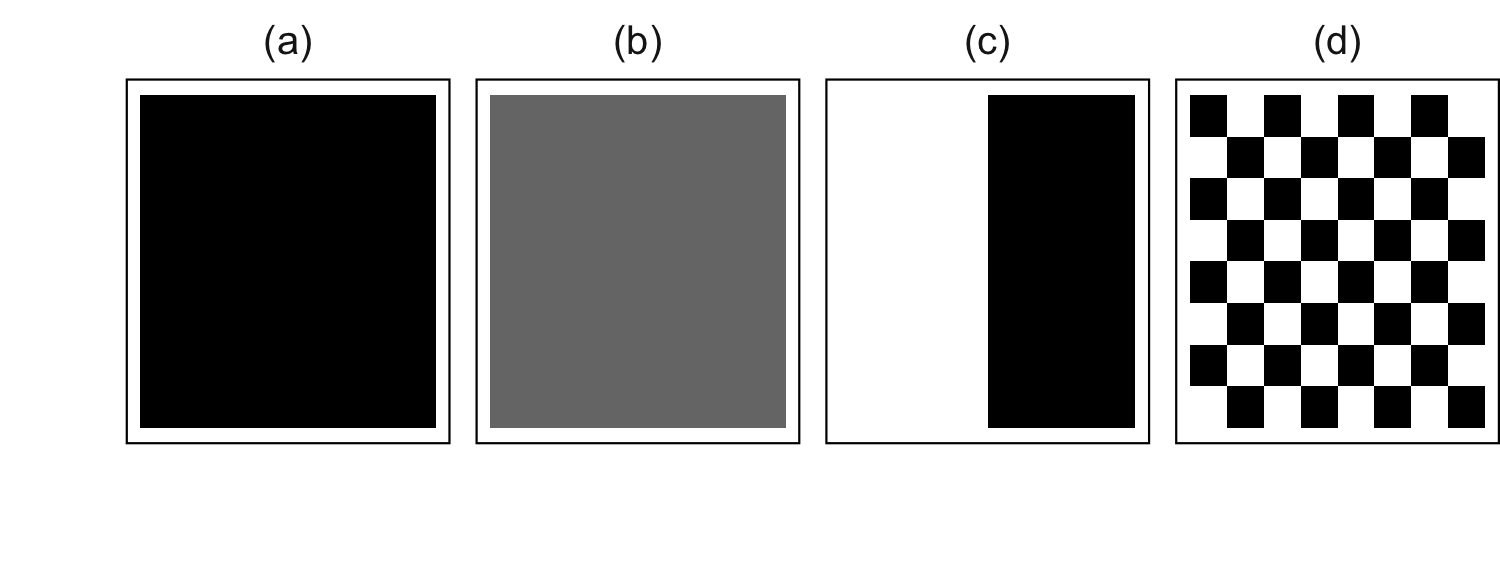
\includegraphics[width=.7\linewidth]{figs/toy.png}
		  \begin{tabular}{c | c c c}
			  City & $H(Y)$ & $I(X,Y)$ & $J(X,Y)$ \\
			  \hline			
			  (a) & 0.0 & 0.0 & 0.0\\
			  (b) & 0.7 & 0.0 & 0.0\\
			  (c) & 0.7 & 0.7 & 0.6\\
			  (d) & 0.7 & 0.7 & 2.7\\
			  \hline  
			\end{tabular}
		\caption{Information theory and the checkboard problem: model cities with various kinds of spatial diversity can be distinguished through progressively more subtle spatial information measures.}
		\label{fig:toy}
		\end{figure}

\section{Methods}
	To motivate our methods, we first consider an idealized problem in which we have a differentiable field $p(y|x)$ of observed probability distributions for each $x \in M \subset \R^n$, where $M$ is intuitively the map on which we work. 

	Fix a point $x_0 \in M$ and a radius $r > 0$. Let $B_r(x_0)$ denote the ball of radius $r$ about $x_0$. Then, define the \emph{local mutual information in radius $r$} as the mutual information between $X$ and $Y$, restricted to the small ball $B_r(x_0)$ about $x_0$:
	\begin{equation}
		I_r(x_0) \triangleq \E_X[D[p(\cdot|X)\| p(\cdot|X \in B_r(x_0))]|X \in B_r(x_0)]
	\end{equation}
	Intuitively, $I_r(x_0)$ measures how much the probability field $p(y|x)$ varies with $x$ in a small neighborhood of $x_0$. It is therefore a natural measure of local complexity, aligned in approach with the global mutual information but designed to detect pattern in local variations. $I_r(x_0) = 0$ if and only if $p(y|x)$ is constant for each $y$ in the ball $B_r(x_0)$, corresponding to a complete lack of local compositional complexity. 

	\begin{figure}
		\centering
		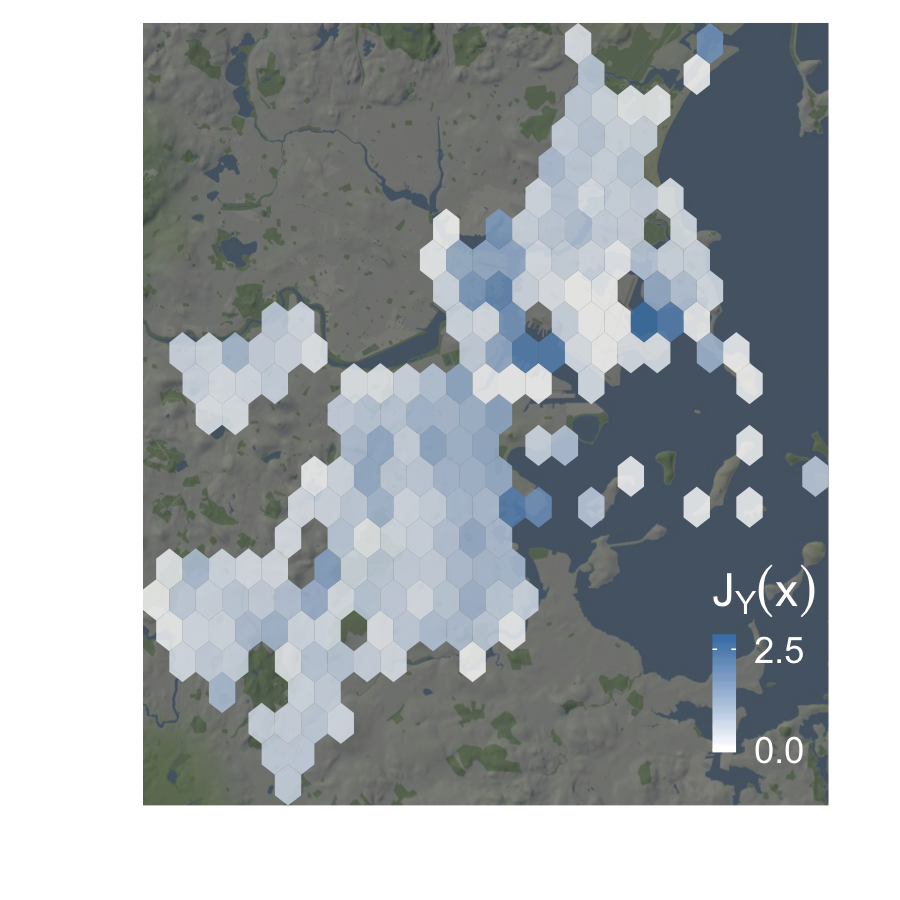
\includegraphics[width=.5\textwidth]{figs/method.png}
		\caption{Illustration of methodology for estimating local information in Suffolk County, MA (Boston). We first cover the map in a hexgrid, and compute the mutual information within each hex from the Census tracts that overlap the hex, weighted by density. }
		\label{fig:method}
	\end{figure}

	In this definition, $r$ may be thought of as the spatial resolution at which we conduct analysis, and $I_r(x_0)$ is highly dependent on $r$. However, it is possible to show that $I_r(x_0)$ is related to a fundamental statistical property of the probability field $p(y|x)$ that is resolution-independent. Under the stated conditions, the following approximation holds: 

	\begin{equation}
		\frac{I_r(x)}{r^2} \cong \frac{1}{4} \text{trace} (J_Y(x))\;, \label{approx}
	\end{equation}
	where $J_Y(x)$ is the Fisher information matrix in $Y$ about $x$, defined as 
	\begin{equation}
		J_Y(x) \triangleq \E\left[ (\nabla_x \log p(y|x))(\nabla_x \log p(y|x))^T \right]\;.
	\end{equation}
	A more formal statement and proof of \eqref{approx} are provided in Appendix 2. The Fisher information $J_Y$ is a fundamental quantity in statistics and information theory. From a geometric perspective, $J_Y$ provides the natural intrinsic metric in the geometric space of probability distributions parameterized by the spatial variable $x$. Equation \eqref{approx} therefore expresses a relationship between the local mutual information $I_r(x)$ and the information geometry of the underlying probability field. Corresponding to the fact that $I_r(x_0)$ vanishes if and only if $p(y|x)$ is constant in $B_r(x_0)$, $J_Y(x_0) = 0$ if and only if $\nabla_x p(y|x_0) = 0$ for all $y$. This implies that $x_0$ is a stationary point, about which the probability field $p(y|x_0)$ exhibits only small (2nd order or smaller) changes with respect to changes in $x$. 

	Since the Fisher information is a strictly local measure of statistical variability around $x$, we can aggregate the Fisher information to derive a measure of average local variability. The \emph{mean local information} is 
	\begin{equation}
	J(X,Y) \triangleq \E_X[\text{trace }J_Y(X)]
	\end{equation} 
	We propose the aggregate quantity $J(X,Y)$ as a third  measure--alongside the entropy $H(Y)$ and mutual information $I(X,Y)$-- as a tool for the information-theoretic structure of spatial compositional complexity. 

\section{Results}
	We assembled block-group level data from the 2008-2012 American Community Survey (ACS), conducted by the U.S. Census Bureau, on race and ethnicity for counties corresponding to 28 large US cities. At this early stage, the counties used were chosen to correspond to the most densely populated urban cores; in future developments we could standardize to conduct analyses for Metropolitan Statistical Areas. We then aggregated the detailed racial and ethnic groups into five meta-categories: `Asian', `Black', `Hispanic', `Other', and `White'. For each city, we computed the entropy $H(Y)$ and the mutual information $I(X,Y)$. To compute the estimated aggregate Fisher information $J(X,Y)$, we tiled the map with a hexagonal grid of cell radius 1km. We then computed the estimated mutual information within each grid cell, and averaged the results weighted by population population. A technical specification of this approach is provided in Appendix 1, and a complete summary of cities and their associated information measures is provided in Appendix 3. 
		
	\begin{figure}
		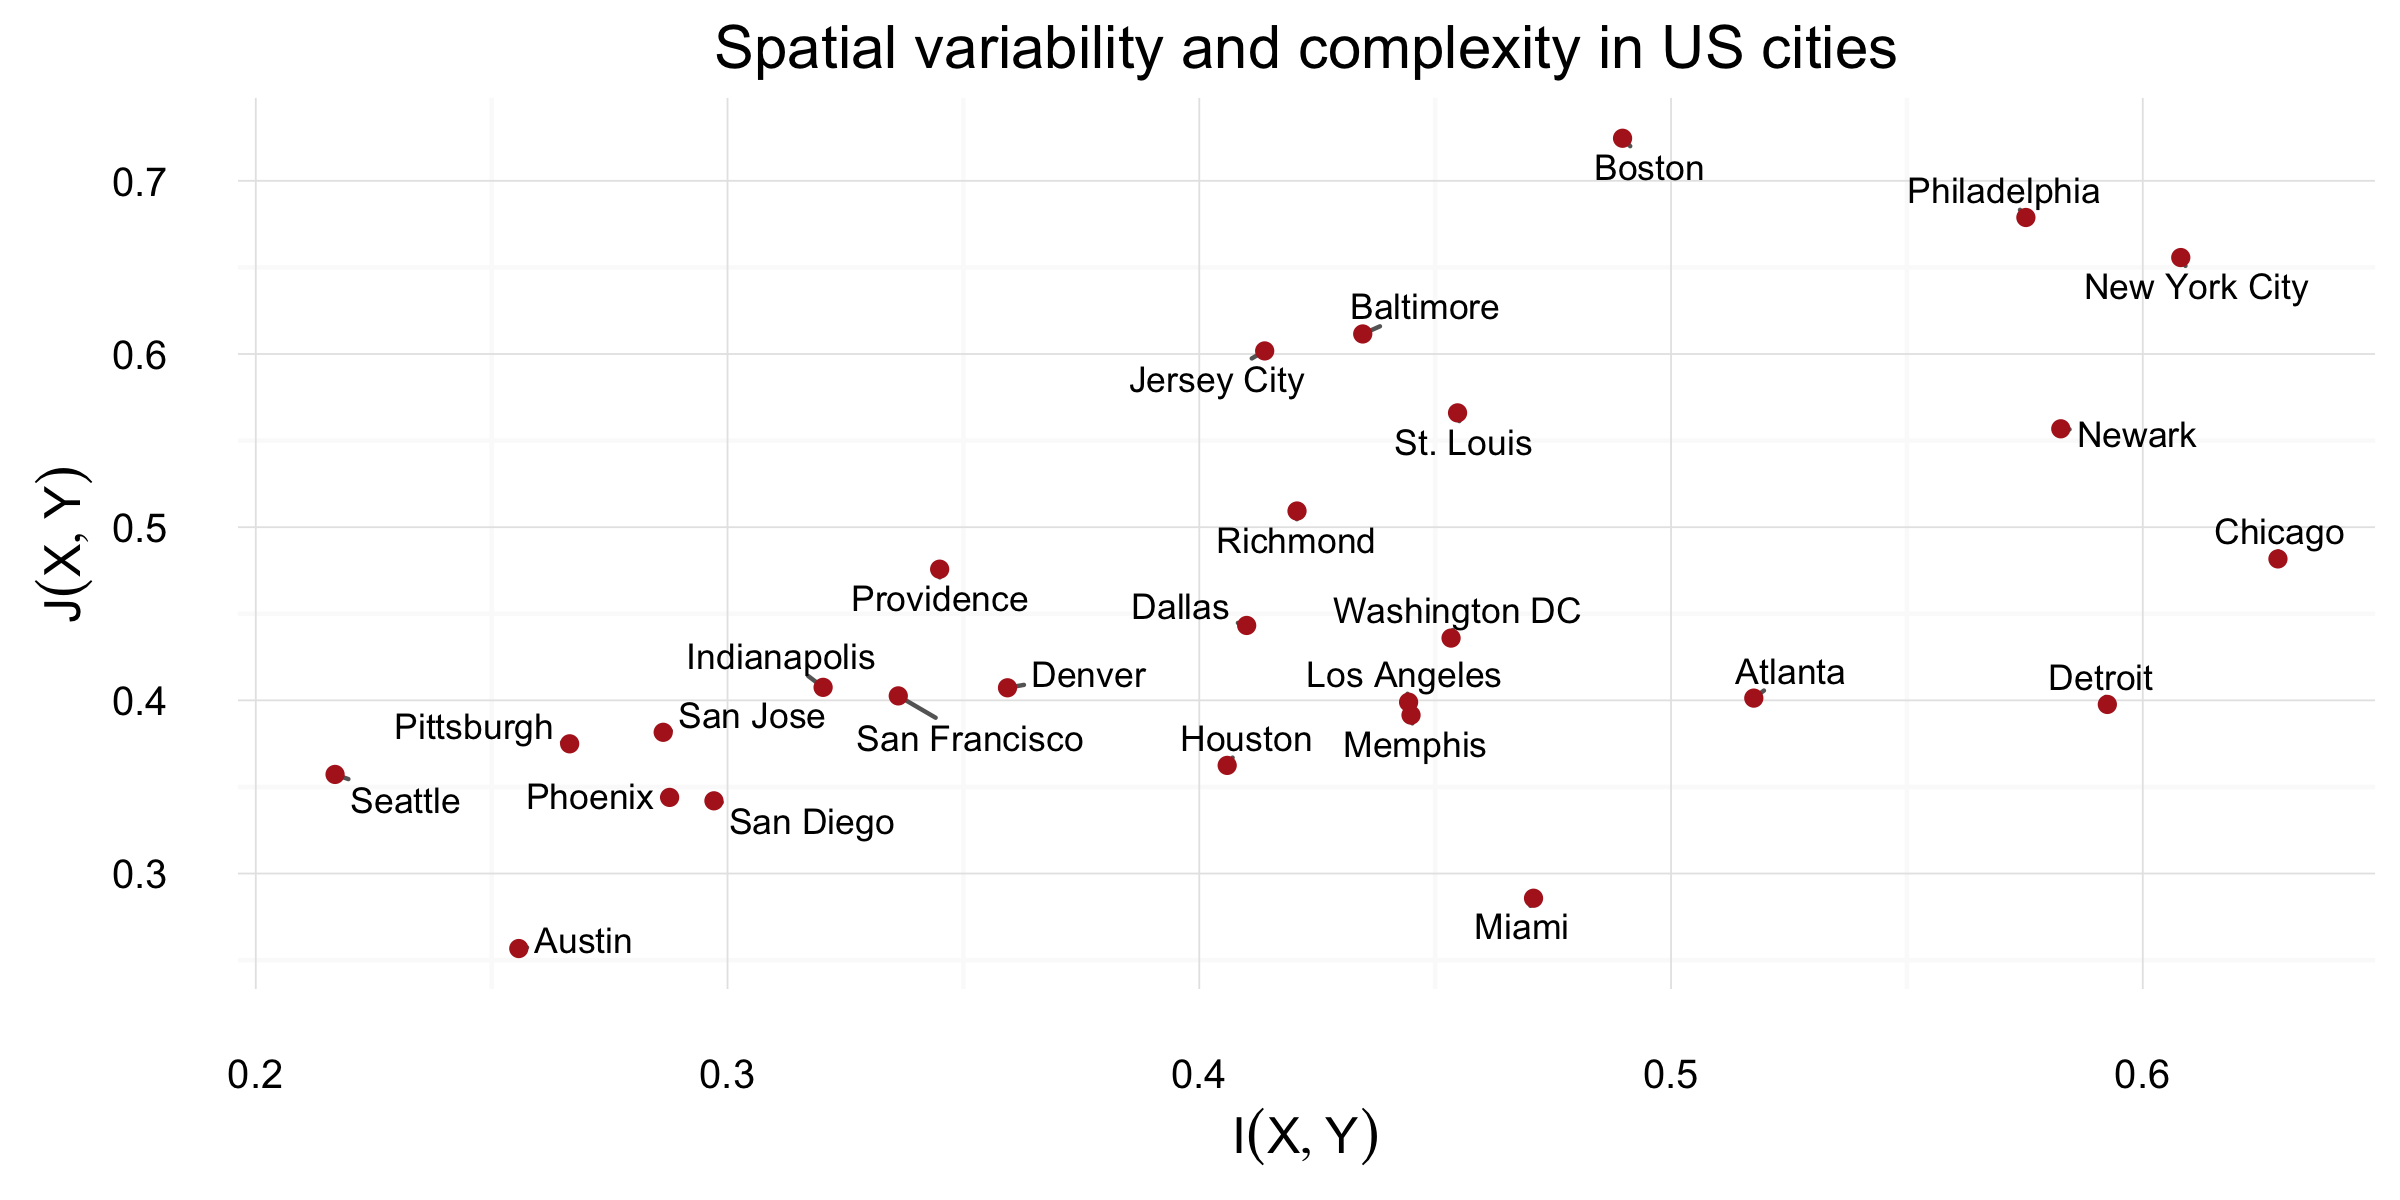
\includegraphics[width=1\textwidth]{figs/mutual_fisher.png}
		\caption{Relationship of global mutual information $I(X,Y)$ and mean local information $J(X,Y)$.} 
		\label{fig:info_cross}
	\end{figure}	
	Figure \ref{fig:info_cross} shows the relationship of the global spatial variability $I(X,Y)$ and mean local variability $J(X,Y)$. An overall positive trend is evident, reflecting the fact that global spatial variability is a prerequisite for local variability: if the city is uniform (like Figure \ref{fig:toy}(a)), then no local differences either exist.  On the other hand, there are substantial variations in $J(X,Y)$ even in cities with comparable global variability $I(X,Y)$. For example, the cities of Detroit and Philadelphia provide a striking contrast. While they have comparable global variability $I(X,Y)$, Philadelphia's $J(X,Y)$ is substantially higher. This reflects the fact that Detroit is composed of large, highly-segregated, monoracial neighborhoods, whereas Philadelphia has a much more fine-grained, intricate neighborhood structure. These patterns illustrate how combinations of the information measures $H(Y)$, $I(X,Y)$, and $J(X,Y)$ can be used to construct taxonomies diversity for American cities. 

	Intriguingly, the mean local variability $J(X,Y)$ appears obey a scaling relation with respect to urban density. In Figure \ref{fig:density}, we plot $J(X,Y)$ against the population density $\rho$ of our studied cities. A clear trend is evident, with $J(X,Y)$ growing linearly with the logarithm of density. We interpret this trend as reflecting a compression of social space in dense urban areas: the same structure of racial variability fits into much less geographical area in New York than in Phoenix. One aspect of diversity in large, dense cities is that one need walk much less distance in order to reach a neighborhood with substantially different racial trends than one's own. 
 
	\begin{figure}
		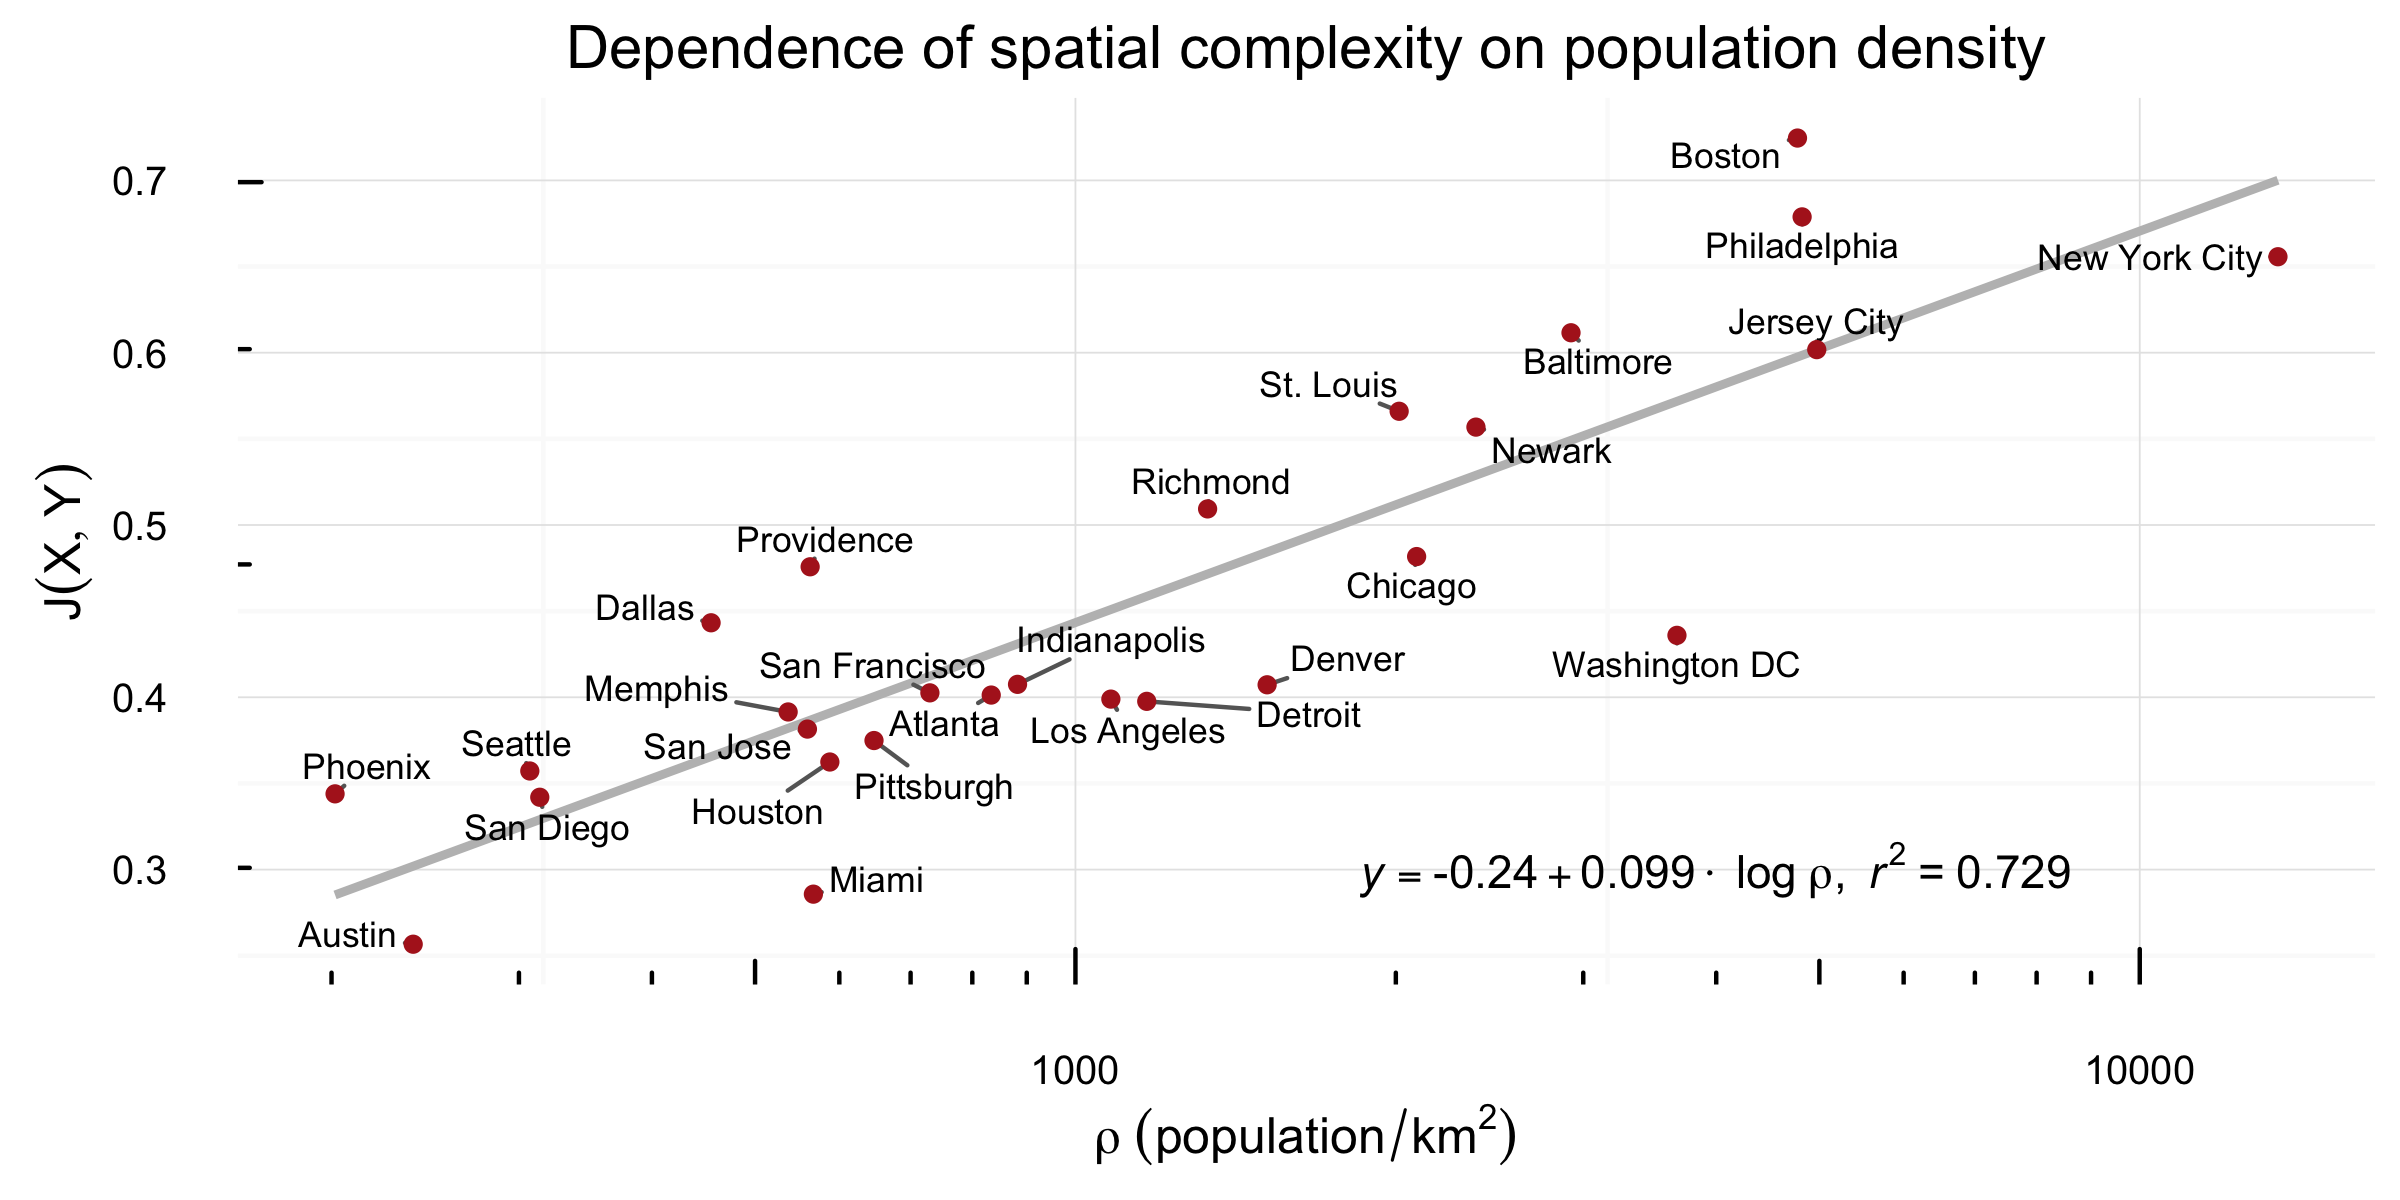
\includegraphics[width=1\textwidth]{figs/density_fisher.png}
		\caption{The mean local information $J(X,Y)$ scales with the logarithm of population density.}
		\label{fig:density}
	\end{figure}	

\section{Discussion}

	We have formulated a novel measure of urban spatial complexity, and applied it to an analysis of spatial distributions of race in American cities. We emphasize that the mean local spatial variability $J(X,Y)$ is novel piece of a more complete information-theoretic characterization that also includes the entropy $H(Y)$ and the global variability $I(X,Y)$. Our results suggest two major directions of further exploration: 

	One major physical question raised by our results is the origin of the scaling relation seen in \ref{fig:density}. This scaling relation may suggest a dynamical process of neighborhood formation and growth common to many American cities. If so, a physical understanding of this process in terms of individual-level behavior is called for. It is tempting to view the scaling relationship as an interplay of spatial preferential attachment and intrinsic limits to neighborhood density due to housing availability, but this view is speculative at this point. A theory to explain this behavior would be most welcome. 

	Another question raised is more operational. In many urban planning contexts, the amount of available data may make direct computations prohibitive. In such contexts, it may be useful to construct a simplifying model of the data the data (such as a clustering) in order to reduce dimensionality and make ``the big picture'' more visible. When a particular demographic phenomenon (such as race) is under consideration, it may be important to ensure that the model preserves the major patterns of variation in the granular data. We conjecture that the local variability $J(X,Y)$ measures the ``model-ability'' of such data sets. Intuitively, a city like Detroit with relatively low $J(X,Y)$ and large, monoracial neighborhoods should be easily representable with relatively few modeled clusters, one for each of the relatively few major neighborhoods. On the other hand, relatively speaking, a city like Philadelphia with very intricate neighborhood structure may require substantially greater model complexity to represent without large loss of information. A promising course of further study is to design an information-theoretic clustering algorithm designed to model urban patterns, and then compare this algorithm's performance to $J(X,Y)$. 

	A third question and final question relates to the time-dependence of spatial structure. On one time scale, daily movement around a city for work or leisure activities has the impact of ``mixing'' separated residents in public spaces, potentially leading to very different spatial patterns of racial difference. On another time scale, these measures may track how the spatial structure of cities evolves over decades, potentially shedding further light on the dynamics of city formation. 		

\bibliography{/Users/phil/bibs/library.bib}{}
\bibliographystyle{plain}
	
\section*{Appendix 1: Computational Methods and Assumptions}
	In this section, we provide a specification of the computational procedure used to estimate $J(X,Y) = \E_x[J_Y(X)]$ using blockgroup level data from the U.S. Census. 

	For fixed Census blockgroup $i$, let $P_i$ be the population, let $A_i$ be the area, let $\rho_i = P_i / A_i$ be the population density, and let $p^i_Y(y)$ be the observed proportion of racial group $y$. For hex $k$ in our hexagonal grid, let $N_k$ be the set of overlapping Census blockgroups. We also define $p^{k}_I(i) = \rho_i / \sum_{i \in N_k} \rho_i$ as the estimated proportion of population within hex $k$ residing in blockgroup $i$. This definition embodies a computationally-simplifying assumption that each blockgroup in $N_k$ overlaps hex $k$ with equal area. Finally, $p^k_Y(y) = \sum_{i \in N_k} p^{k}_I(i) p^i_Y(y)$ is the estimated overall racial composition of hex $k$. Then, we estimate the mutual information in hex $k$ as 
	\begin{equation}
		I(k) = \sum_{i \in N_k} p^k_I(i) D[p^i_Y(\cdot) \| p^k_Y(\cdot)]\;. 
	\end{equation}
	Using \eqref{approx}, the estimated Fisher information is 
	\begin{equation}
		J(k) \approx \frac{4 I(k)}{r^2}
	\end{equation}
	where $r$ is the grid radius. The estimated population in hex $k$ is $P_k = A_k\sum_{i \in N_k} \rho_i$, where $A_k$ is the cell area. We finally estimate $\E_X[J(X)]$ as 
	\begin{equation}
		J(X,Y) = \E_X[J_Y(X)] \approx \frac{1}{\sum_k P_k} \sum_k P_k J(k)
	\end{equation}
\section*{Appendix 2: Relation of Local Mutual Information and Fisher Information}
	In this appendix, we present a rigorous mathematical justification of the claim that the local mutual information approximates a fundamental quantity intrinsic to the distribution $p(Y,X)$. The argument relies on an idealization in which, rather than have a finite, discrete set of observations for each tract, we have a continuous field of observations across the map. The precise statement of this result and its justification follow. 


	Let $X$ be a continuous random variable taking values in $\R^n$, and let $Y$ be a discrete random variable define on finite alphabet $\mathcal{Y}$. Suppose further that $p(y|x) > 0$ and that $p(y|x)$ is differentiable as a function of $x$ for all $x,y \in \R^n \times \mathcal{Y}$. Fix $x_0 \in R^n$, and define $B_r \triangleq B_r(x_0) = \{ x \in R^n \;|\; \norm{x - x_0} \leq r \}$. Additionally, define the \emph{local mutual information} in $B_r$ as
	\begin{equation}
		I_r \triangleq I_r(x_0) \triangleq \E_X[D[p(\cdot|X)\| p(\cdot|X \in B_r)]|X \in B_r]\;.
	\end{equation}
	where $D[p\|q] = \sum_{y} p(y) \log \frac{p(y)}{q(y)}$ is the Kullback-Leibler divergence of $q$ from $p$. 

	\begin{thm} \label{thm1}
		Under the stated conditions, 
		\begin{equation}
			\lim_{r\rightarrow 0} \frac{I_r(x_0)}{r^2} = \frac{n}{2(n+2)} \emph{trace}\; J_Y(x_0)\;.
		\end{equation}
		where the Fisher information $J_Y(x_0)$ is 
		\begin{align}
		J_Y(x) &\triangleq \E\left[\nabla_x S_{Y}(x)\nabla_x S_{Y}(x)^T \right] \\
		S_y(x) &\triangleq \log p(y|x)\;.
	\end{align}
	\end{thm}
	The proof of Theorem \ref{thm1} proceeds by the application of a number of Taylor approximations, in tandem with a fundamental relationship of information geometry. We first expand out $I_r$ explicitly as
	\begin{equation}
		I_r = \int_{B_r} p(x|X \in B_r) D[p(\cdot|x)\| p(\cdot|X \in B_r)] d^n x\;. \label{eq:explicit}
	\end{equation}

	\begin{lm} \label{approximations}
		The following approximation relationships hold for the components of \eqref{eq:explicit}:
		\begin{enumerate}[label=\emph{(\alph*)}]
			\item $p(X\in B_r,Y) = p(x_0, Y) v(B_r) + O(r^{n+2})$
			\item $p(Y|X \in B_r) = p(Y|x_0) + e_y$ where the error terms $e_y$ satisfy $e_y \in O(r^{2})$ and $\sum_{y \in \mathcal{Y}} e_y = 0$. 
			\item $p(x|X \in B_r) $
		\end{enumerate}
	\end{lm}
	\begin{proof}
		For each approximation,  we directly apply Taylor expansions about $X = x_0$. 
		\begin{enumerate}[label=(\alph*)]
			\item We have 
				\begin{align}
					p(X\in B_r, Y) &= \int_{B_r} p(x,Y) \; d^nx \\
					&= \int_{B_r} p(x_0,Y) + \frac{\partial p(x_0, Y)}{\partial x}(x - x_0) + O(\norm{x - x_0}^2) \; d^nx \\
					&= p(x_0, Y)v(B_r) +  \frac{\partial p(x_0, Y)}{\partial x} \int_{B_r} (x - x_0)\; d^nx  \\
					&\quad \quad+ O\left(\int_{B_r} \norm{x - x_0}^2\; d^nx\right) \\
					&= p(x_0, Y)v(B_r) + O(r^{n+2})\;,
				\end{align}
				where the middle term vanishes due to spherical symmetry. 
			\item The fact that the error terms $e_y$ must satisfy $\sum_{y \in \mathcal{Y}} e_y = 0$ follows from the fact that $p(Y|X \in B_r)$ must be a valid probability distribution over $\mathcal{Y}$. We'll now show that $e_y \in O(r^{ß2})$. First, 
				\begin{align}
					p(X \in B_r) &= \sum_{y\in \mathcal{Y}} p(X \in B_r, y)  \\
					&= \sum_{y\in \mathcal{Y}} \left[p(x_0, y)v(B_r) + O(r^{n+2}) \right] \\
					&= p(x_0)v(B_r) + O(r^{2});\,
				\end{align}
			from part (a). Next, 
				\begin{align}
					p(Y|X \in B_r) &= \frac{p(X\in B_r, Y)}{p(X \in B_r)} \\
					&= \frac{p(x_0, Y)v(B_r) + O(r^{n+2})}{p(x_0)v(B_r) + O(r^{n+2})} \\
					&= p(Y|x_0) + O(r^2)\;,
				\end{align}
			which completes this part of the argument. 
			\item First, 
				\begin{align}
					p(X \in B_r) &= \int_{B_r} p(x) \; d^nx  \\
					&= \int_{B_r} \left[p(x_0) + \nabla p(x_0)(x - x_0) + O(r^2)\right] \; d^nx \\ 
					&= p(x_0) v(B_r) + O(r^{n+2})\;,
				\end{align}
				where the middle term again vanishes through sphericla symmetry. Thus, for $x \in B_r$, we have
				\begin{align}
					p(x | X \in B_r) &= \frac{p(x)}{p(X \in B_r)} \\
					&= \frac{p(x_0) + \nabla p(x_0)(x - x_0) + O(r^2)}{p(x_0) v(B_r) + O(r^{n+2})} \\
					&= \frac{1 + O(r)}{v(B_r)}\;.
				\end{align}
		\end{enumerate}
	\end{proof}

	\begin{lm} The following approximation holds for the divergence factor in the integral \eqref{eq:explicit}
		\begin{equation}
			D[p(\cdot|x)\| p(\cdot|X \in B_r)] = D[p(\cdot|x)\| p(\cdot|x_0)] + O(r^{3})
		\end{equation}
	\end{lm}
	\begin{proof}
		We compute directly: 
		\begin{align}
			D[p(\cdot|x)\| p(\cdot|X \in B_r)] &= \sum_{y \in \mathcal{Y}} p(y|x) \log \frac{p(y|x)}{p(y|X \in B_r)} \\
			&= - H[Y|X = x] - \sum_{y \in \mathcal{Y}} p(y|x) \log p(y|X \in B_r) \\
			&= - H[Y|X = x] - \sum_{y \in \mathcal{Y}} p(y|x) \log \left(p(y|x_0) + e_y)\right) \tag{from Lemma \ref{approximations}}\\
			&= - H[Y|X = x] - \sum_{y \in \mathcal{Y}} p(y|x) \left[\log p(y|x_0) + \frac{e_y}{p(y|x_0)} + O(e_y^2)\right] \\
			&= D[p(\cdot|x)\| p(\cdot|x_0)] + \sum_{y \in \mathcal{Y}} \frac{p(y|x)}{p(y|x_0)}  e_y \tag{quadratic terms negligible} \\
			&=D[p(\cdot|x)\| p(\cdot|x_0)] \\
			&\quad + \sum_{y \in \mathcal{Y}} \left(1 + \frac{1}{p(y|x_0)} \nabla p(y|x_0)(x - x_0) + O(r^{2})\right)    e_y \\
			&= D[p(\cdot|x)\| p(\cdot|x_0)] + \sum_{y \in \mathcal{Y}} \left[e_y + O(r^{3})\right] \tag{$e_y \in O(r^2)$}\\
			&= D[p(\cdot|x)\| p(\cdot|x_0)] + O(r^3) \tag{$\sum_{y \in \mathcal{Y}} e_y = 0$}
		\end{align}
	\end{proof}

	\begin{lm} For any positive-semidefinite matrix $A \in \R^{n\times n}$, 
		$$\int_{B_r} \left< x - x_0, A(x-x_0) \right> d^n x = \frac{n}{n+2} r^{2} v(B_r) \text{\emph{trace}} (A)$$
	\end{lm}
		
	\begin{proof}
		Since $A$ is positive-semidefinite, there exist an orthonormal matrix $P$ and a diagonal matrix $D$ such that $A = P^TDP$. Furthermore, the entries of $D$ are the eigenvalues $\{\lambda_i\}$ of $A$. Then, 
		\begin{align}
			\int_{B_r} \left< x - x_0, A(x-x_0) \right> d^n x &= \int_{B_r} \left< x - x_0, P^T DP(x-x_0) \right> d^n x\\
			&= \int_{B_r} \left< P(x - x_0),  DP(x-x_0) \right> d^n x \;.
		\end{align}
		We can regard $P$ as a reparameterization of $B_r$; since $\det P = 1$, we have 
		\begin{align}
			\int_{B_r} \left< P(x - x_0),  DP(x-x_0) \right> d^n x &= \int_{B_r} \left< x - x_0,  D(x-x_0) \right> d^n x \\
			&= r^n\int_{B_n} \left< rx, rDx \right> d^n x \\
			&= r^{n+2}\int_{B_n} \left< x, Dx \right> d^n x \;,
		\end{align}
		where $B_n$ is the unit $n$-ball. We also let $S_n(r)$ be the $n$-sphere of radius $r$. Continuing, 
		\begin{align}
			r^{n+2}\int_{B_n} \left< x, Dx \right> d^n x &= r^{n+2} \int_{B_n} \sum_{i= 1}^n x_i^2 \lambda_i \; d^nx \\
			&= r^{n+2} \sum_{i = 1}^n \lambda _i \int_{B_n} x_i^2 \; d^nx \\
			&= \frac{r^{n+2}}{n} \sum_{i = 1}^n \lambda _i \int_{B_n} \norm{x}^2 \; d^nx \\ \tag{spherical symmetry} \\
			&= \frac{r^{n+2}}{n} \text{trace}(A)  \int_{B_n} \norm{x}^2 \; d^nx \\ \tag{spherical symmetry} \\
			&= \frac{r^{n+2}}{n} \text{trace} (A) \int_{\rho \in [0,1]} \rho^2 S_{n-1}(\rho) d\rho \\
			&= \frac{r^{n+2}}{n} \text{trace} (A) \int_{\rho \in [0,1]} \rho^{n+1} S_{n-1}(1) d\rho \\
			&= \frac{r^{n+2}}{n} \text{trace} (A)  \frac{1}{n+2} S_{n-1}(1) \\
			&= \frac{r^2}{n+2}  \text{trace} (A)  n r^{n}v(B_n(1)) \\
			&= \frac{n}{n+2} r^{2} v(B_r) \text{trace} (A)\;,
		\end{align}
		as was to be shown. 
	\end{proof}

	\begin{fct*}
		The Kullback-Leibler divergence and the Fisher information $J_Y$ are related according to the approximation 
		\begin{equation}
			D[p(\cdot|x)\| p(\cdot|x_0)] = \frac{1}{2}\left<x - x_0, J_Y(x_0)(x - x_0) \right> + O(\norm{x - x_0}^3)
		\end{equation}
	\end{fct*}

	We are finally ready to prove Theorem \ref{thm1}. Computing directly, we have 
	\begin{align}
		I_r(x_0) &\triangleq \E_X[D[p(\cdot|X)\| p(\cdot|X \in B_r)]|X \in B_r]\;. \\
		&= \int_{B_r} p(x|X \in B_r) D[p(\cdot|x)\| p(\cdot|X \in B_r)] d^n x \\
		&= \int_{B_r} \left[\frac{1 + O(r)}{v(B_r)}\right] D[p(\cdot|x)\| p(\cdot|X \in B_r)] d^n x \tag{Lemma 1(c)}\\ 
		&= \left[\frac{1 + O(r)}{v(B_r)}\right]\int_{B_r}  \left(D[p(\cdot|x)\| p(\cdot|x_0)] + O(r^{3})\right) d^n x \tag{Lemma 2}\\
		&= \left[\frac{1 + O(r)}{v(B_r)}\right]\int_{B_r} \left( \frac{1}{2}\left<x - x_0, J_Y(x_0)(x - x_0) \right> + O(\norm{x - x_0}^3) + O(r^{3})\right) d^n x \\
		&= \frac{1}{2}\left[\frac{1 + O(r)}{v(B_r)}\right]\int_{B_r} \left(\left<x - x_0, J_Y(x_0)(x - x_0) \right> + O(r^{3})\right) d^n x \\
		&= \frac{1}{2}\left[\frac{1 + O(r)}{v(B_r)}\right]\left(\frac{n}{n+2} r^{2} v(B_r) \text{trace} (J_Y(x_0)) + v(B_r)O(r^{3})\right) \\
		&= r^2\frac{n}{2(n+2)}\left[1 + O(r)\right]\left(\text{trace} (J_Y(x_0)) + O(r^{3})\right)\;.
	\end{align}
	Dividing through by $r^2$ and computing the limit as $r \rightarrow 0$ proves the result. 
\section*{Appendix 3: Table of Information Measures for Cities Studied}
	The table below is sorted  by the population density of the city studied. 
	\begin{tabular}{l c c c c }%
	    \bfseries City & Density (km$^{-2}$) & $H(Y)$ & $I(X,Y)$ & $J(X,Y)$ 
	    \csvreader[head to column names]{figs/table.csv}{}% use head of csv as column names
	    {\\\hline\City & \Density & \HY & \IXY & \J}% specify your coloumns here
    \end{tabular}






\end{document}